\chapter{Related Work}
\label{cha:relatedwork}

This section introduces the reader to the state of the art of existing literature on human mobility patterns, approaches to stop detection and network graph analysis.

\section{Human Mobility within the city}
\label{cha:introduction_hummob}

Understanding of human mobility patterns is essential for implementing various environmental changes \cite{HumanMobility2}, assessing and improving existing mobile network protocols \cite{HumanMobility1} or to learn significant locations and build movement prediction models \cite{StopDet1}. 

The study \cite{HumanMobility1} points out that it is more human intentions instead of geographical factors which produce heavy-tailed distribution of human mobility (human tend to move by about similar distance from point to point, with heavy tailed exceptions). It also assumes, that this is caused by the power-law tendency of popularity of locations people visit or simply human interests. The study confirms, along with the other study \cite{HumanMobility2}, that both walking distance and walk duration follows heavy tailed distribution, where the average walking speed in the city for man aged 40 is 1.4 m/s (5 km/h), and slowest one is for elderly (with walking impairment) below 1 m/s (3.6 km/h) \cite{HumanMobility3}. 

We find, that analyzing human mobility on short distances might be important for approaches to stop detection. 

\section{Approaches to stop detection for location-based services}
\label{cha:introduction_appr_stopdet}

The state of the art within works in the area of learning significant places for people usually implies usage of some sort of stop detection algorithm, which is usually bound to the way how the data is being acquired from mobile devices and the technology behind acquisition process. 

As an example, study \cite{StopDet2} proposed approach based on geo-grid of cells and continuous GSM trajectories matching certain cells. As a predicate for assuming a stay at certain cell, simple duration threshold has been used. Furthermore, post processing in the form of significance mining has been applied to extract only the most important places for the certain user and filter less significant ones. 

Similar approach, however using continuous GPS trajectories, targets at finding places where user
spends their time. Their assumption was that mobile device outside of building generates location data until the user enters a building, resulting in a time gap between recorded locations. To pre-filter short stays at location, duration threshold has been used. Using clustering concept, they find the significant places out of pre-filtered data.  

In the paper \cite{MobilityIndexGIS}, non-continuous position acquisition technique is used and movement of mobile devices between cells (handovers) is considered. To detect the periods of slow movements of stops at the specific location, parameter called Mobility Index is considered. 

\begin{figure}[!ht]
	\centering
	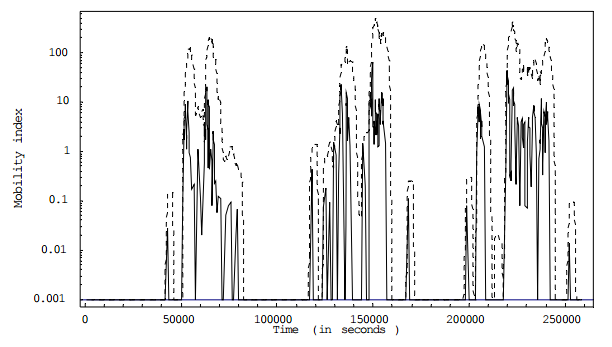
\includegraphics[width=0.8\textwidth]{images/intro_mobility_index.png}\\
	\caption{Mobility Index. Source: \cite{MobilityIndexGIS}}
	\label{fig:introduction_mob_index}
\end{figure}

In the areas with many GSM cells (mainly areas with high population density), the mobile
terminal may change cells frequently (which might identify movement) or stay at one cell for longer time. Given a set of consecutive records, the mobility of a user can be estimated by calculating the Mobility Index over a pre-defined time period (sliding window). The Mobility Index is defined as the sum of the "distances" between each record and the previous ones, where the "distance" is the inverse of the time spent on each cell. If the value of the index is below a certain threshold, it is assumed that the object stopped or moved slowly. In the publication, sliding window of 10 minutes and a mobility index threshold value of 6 has been used for certain area. The obtained results were in agreement with actual movements during more than 90\% of the time.

Rapid drop in mobility index represents a set of points (restricted area) in which user has been moving slowly or stopped. Increase in mobility index means that user changed position from restricted area and is moving.

\section{Clustering}

Clustering can be described as "\textit{the task of grouping a set of objects in such a way that objects in the same group (called a cluster) are more similar (in some sense or another) to each other than to those in other groups (clusters)}" \cite{clustering}. 

There are different types of clustering (such as centroid, distribution, or density-based), and different algorithms with parameters that can be applied (such as K-means, DBSCAN, or OPTICS). However, they all work to achieve the same goal of structuring (clustering, grouping) similar objects and neglecting outliers from these groups. The algorithm and parameters are application sensitive and can produce highly different clusters. The difficulty of DBSCAN is figuring out the two parameters, the minimum points per cluster (\textit{minPts}) and the radius of the clusters (\textit{eps}).

\begin{figure}[!ht]
	\centering
	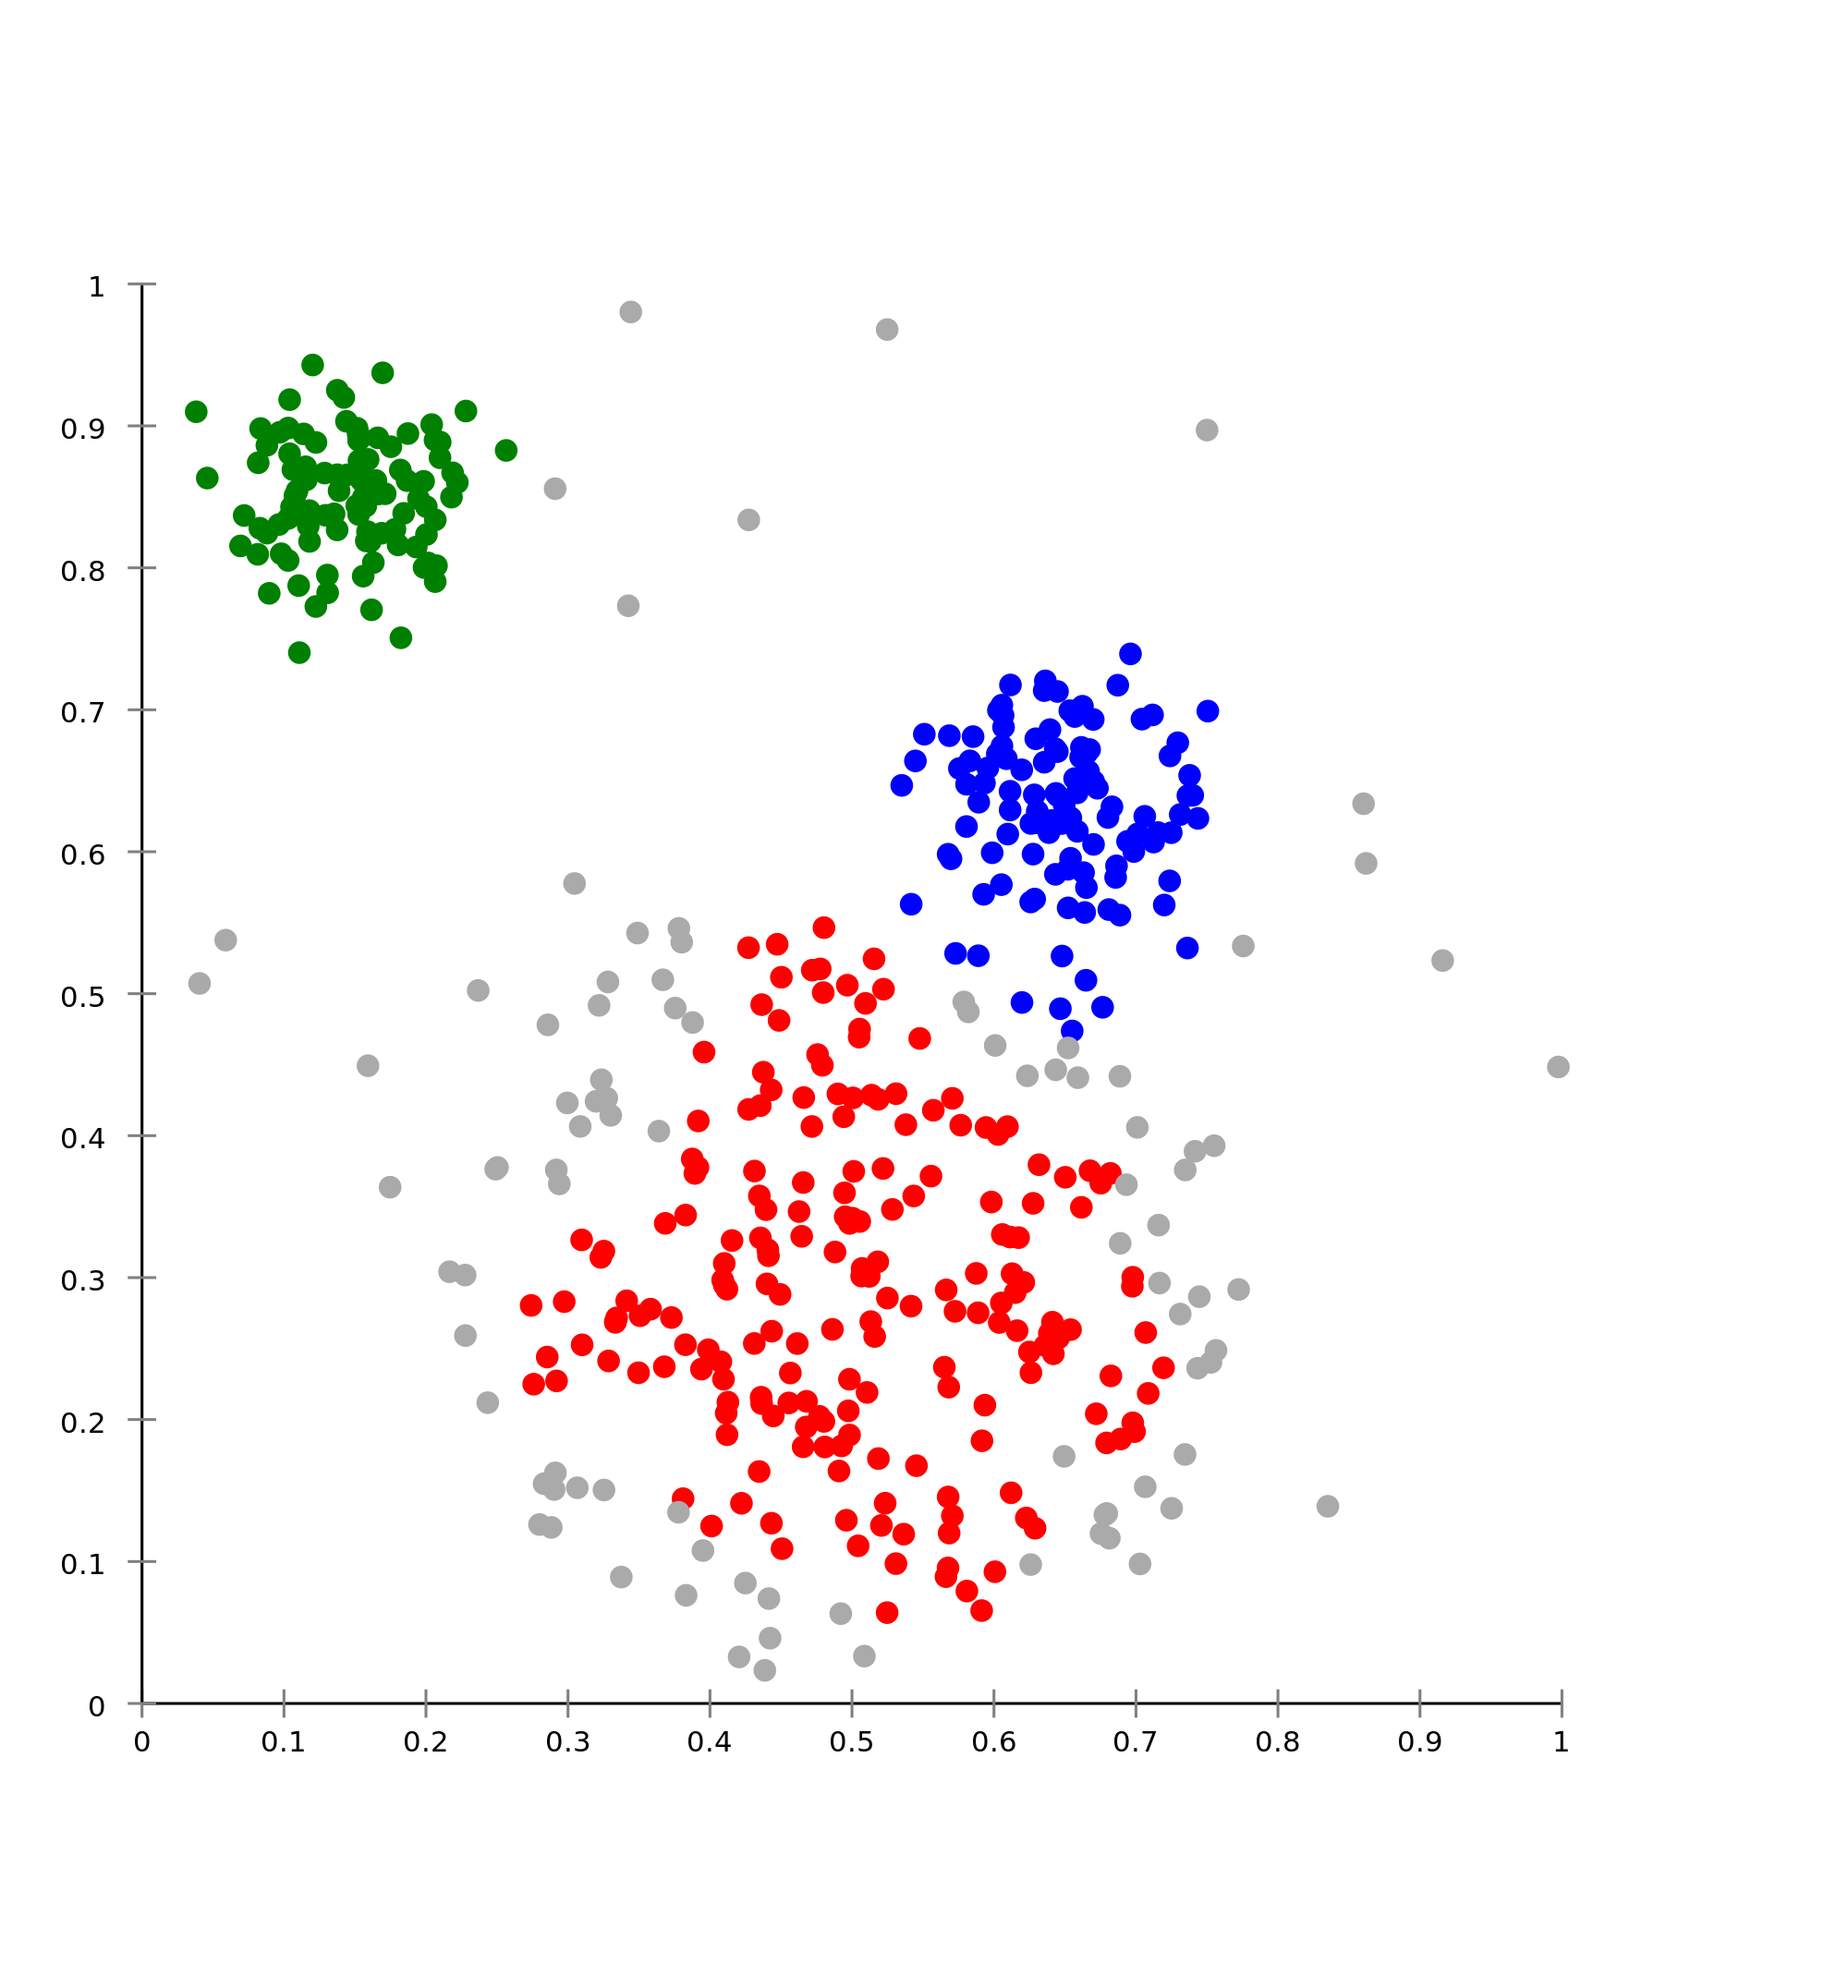
\includegraphics[width=0.5\textwidth]{images/clustering.png}
	\caption{ Clustering applied to a dataset. }
	\label{fig:clustering}
\end{figure} 

\subsection{DBSCAN on spark}

 In this project we used an implementation of the DBSCAN clustering algorithm on top of Apache Spark. The imp,enetation is called DBSCAN on Spark \cite{dbscan_on_spark} and loosely based on the paper from \textit{He, Yaobin, et al. "MR-DBSCAN: a scalable MapReduce-based DBSCAN algorithm for heavily skewed data"}.
 
  This implementation of DBSCAN runs in parallel by splitting the data space into boxes, using the number of boxes as a cost estimator for the algorithm. Each box then grows to include one \textit{eps} in it. After each box and its points has been determined the traditional DBSCAN algorithm is run on the points in each box. Finally it examines the intersection points betweeen boxes and merges the result together \cite{vis_dbscan_on_spark}. See figure set \autoref{fig:dbscan_on_spark} for a visual guide. 
 
\begin{figure}
	\centering
	\begin{minipage}{.5\textwidth}
		\centering
		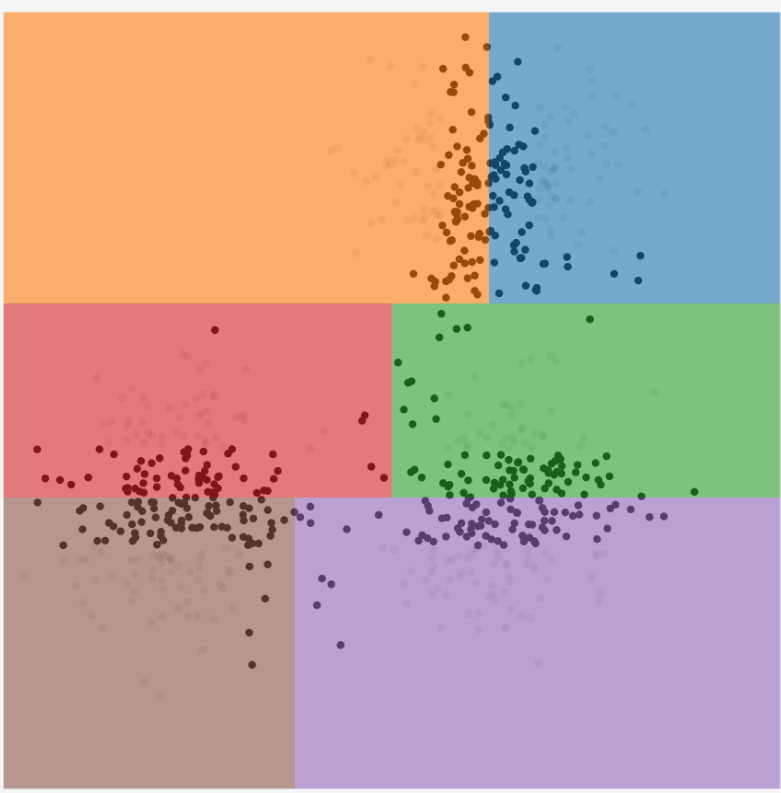
\includegraphics[width=.6\linewidth]{images/db1_c.png}
		\captionof{figure}{Step 1. DBSCAN on Spark assign the data space into boxes.}
		\label{fig:db1_c}
	\end{minipage}%
	\begin{minipage}{.5\textwidth}
		\centering
		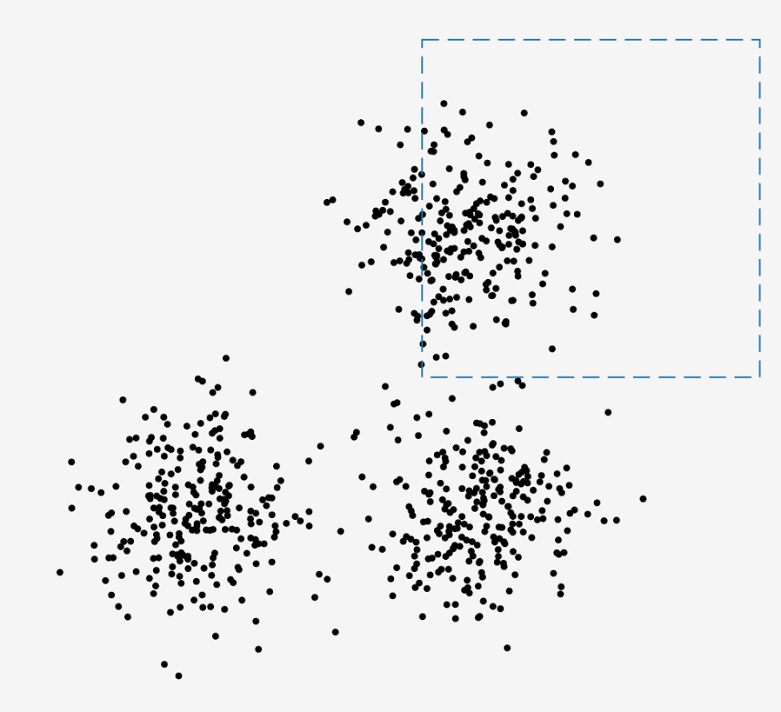
\includegraphics[width=.6\linewidth]{images/db2_c.png}
		\captionof{figure}{Step 2. Each box grows to include the points that are within one \textit{eps} of it.}
		\label{fig:db2_c}
	\end{minipage}
	\begin{minipage}{.5\textwidth}
		\centering
		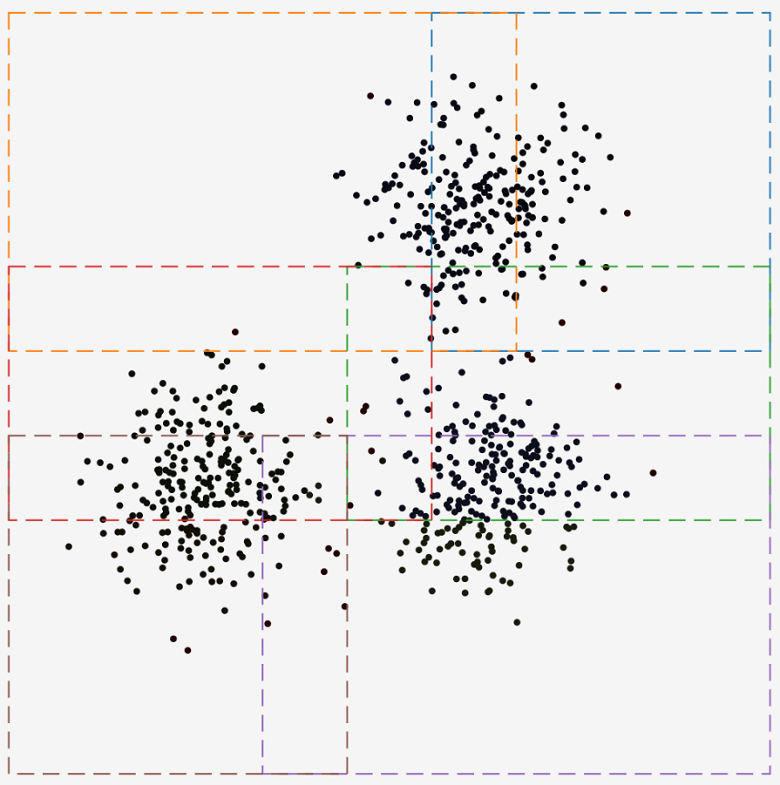
\includegraphics[width=.6\linewidth]{images/db3_c.png}
		\captionof{figure}{Step 3. Traditional DBSCAN algorithm is applied in parallel for each box. Each different color represents a different cluster. }
		\label{fig:db3_c}
	\end{minipage}%	
	\begin{minipage}{.5\textwidth}
		\centering
		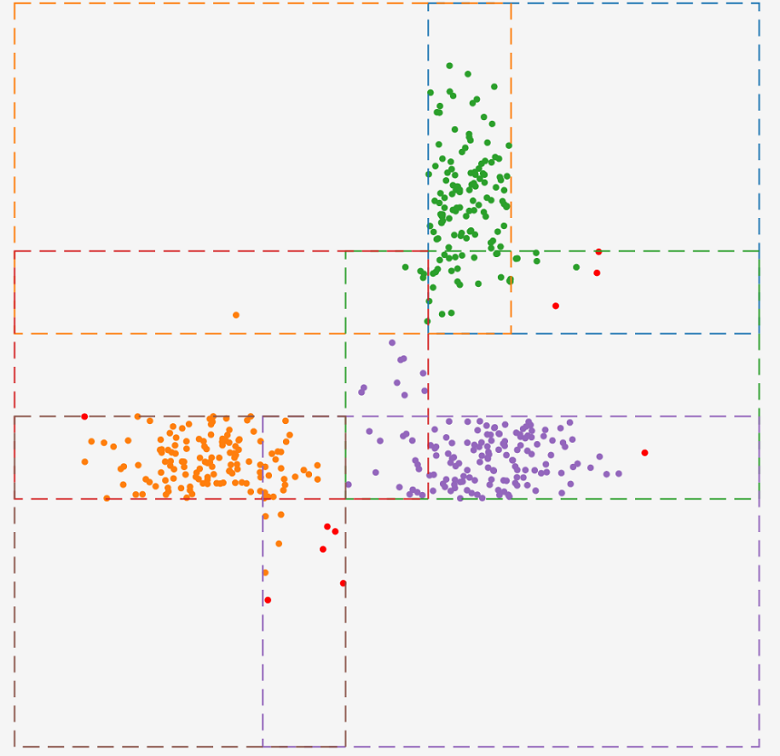
\includegraphics[width=.6\linewidth]{images/db4_c.png}
		\captionof{figure}{Step 4. After DBSCAN is done, all points within the borders of two clusters are examined. If they are part of a cluster within two boxes they are merged to one cluster. }
		\label{fig:db4_c}	
	\end{minipage}		
	\begin{minipage}{.5\textwidth}
		\centering
		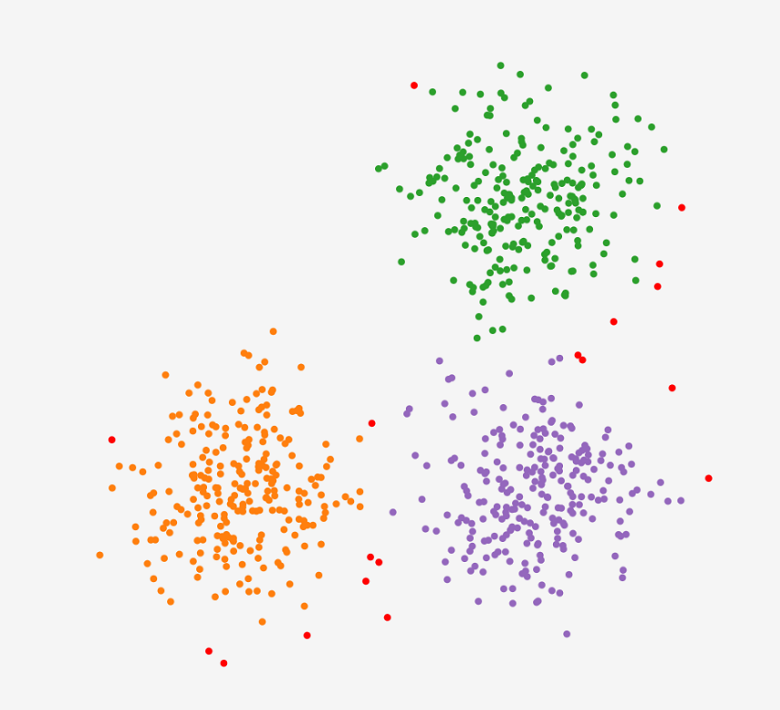
\includegraphics[width=1\linewidth]{images/db5_c.png}
		\captionof{figure}{Step 5. Finally all remaining points are labelled with the global identified cluster and we are done. (red points are noise points). }
		\label{fig:db5_c}	
	\end{minipage}%
	\captionof{figure}{DBSCAN on Spark \cite{vis_dbscan_on_spark}, maintained by Irving Cordova. }
	\label{fig:dbscan_on_spark}
\end{figure}
\FloatBarrier

\section{Graph Analytics: For analyzing human mobility data}
\label{cha:graphrelatedworks}
Graph based models are very commonly used in scientific research related to mobility data. Graph analytics is used to study the relationships between nodes and edges in a network. It helps identify key players in a network, areas of interest, even differentiate between usual and unusual patterns in the data. In this section we present research papers that have used concepts of graph analytics and influenced our work. 

One of the most important concepts for analyzing mobility data is an Origin-Destination Matrix(OD). OD matrix and hotzones have been used in the study to analyze urban population migration based on data from Beijing taxi service. The study was presented in the paper \cite{zhu2013urban}. The authors identified hotzones in the city of Beijing by analyzing the most popular pickup and drop points from the trip data. They also analyzed the OD pairs to identify most frequent movement patterns of the residents. Their findings corroborate with their assumptions and some of the most important areas (key transport facilities/financial hubs) got identified as the hotzones. 

In a similar study, based on taxi data from Berlin \cite{bischoff2015analysis}, the authors used OD Matrix to compute location-based taxi demand in Berlin. They analyzed time and location based taxi demand patterns, e.g. how the demand pattern varies for the two airports in Berlin. They computed the top 100 OD-relations and analyzed the attractiveness of each route. The study identified important places in the city as the most common destinations.


OD matrix is also used for travel demand estimation problems. In the paper \cite{ma2013deriving}, the authors have used mobile phone data of users, based on their daily activity and path choices of users, for their analysis. This data has been used to derive sample OD matrices and subsequently used for traffic assignment.


Apart from human mobility data, graph based models are also very useful for analyzing air traffic as discussed in the paper \cite{marzuoli2011two}. The authors discussed a two step based process for building the network graph based on air traffic. In their study, Marzuoli et al. created a network flow model of the airspace. They defined their network as a system of nodes and directed edges. Working with air traffic, they defined network nodes as areas where aircraft are entering or leaving a region and edges as flow corridors used by the aircrafts. This data was used to create origin-destination pairs to determine relative importance of different routes used by aircrafts.

The concepts of OD Matrix, hotspot identification, and modelling raw data into a graph, as are of primary importance for our work.